\documentclass[a4paper]{article}
\usepackage{polski}
\usepackage[utf8]{inputenc}
\usepackage{enumerate}
\usepackage{hyperref}
\usepackage{graphicx}
\usepackage{float}
\author{}

\title{Roboty mobilne - I kamień milowy}
\date{}

\begin{document}
\maketitle

\begin{enumerate}

\item Skład grupy:

Dominik Hebda 209168 \\
Filip Malinowski 209193

\item Silniki:

Do budowy rękawicy egzoszkieletu zastosujemy bezrdzeniowe silniki prądu stałego. Najmniejsze silniki jakie można dostać mają wymiary
\begin{math}
4mm \cdot 8mm.
\end{math}
Do naszego projektu użyjemy silników podobnych lub trochę większych rozmiarów. Zostanie to ustalone po wykonaniu komputerowego modelu rękawicy. Prawdopodobnie zastosujemy przekładnię 3:1. To również doprecyzujemy po wykonaniu obliczeń. Przy odłączonym zasilaniu silniki będą pracować w rękawicy jako prądnice. Na każdy palec użyjemy 4 silników. Prąd silników będzie w zakresie od 0.23A do 0.85A przy zasilaniu 3V.

\item Warstwa sprzętowa:

Do realizacji oprogramowania rękawicy skorzystamy z mikrokontrolera
\href{http://www.microchip.com/wwwproducts/en/PIC18F4431}{PIC18F4431}.
Jeden mikroprocesor będzie obsługiwać jeden palec rękawicy. W mikrokontrolerze wykorzystamy osiem kanałów PWM, osiem pinów GPIO oraz 8 kanałów przetwornika ADC. Do sterowania silnikami w jednym palcu wykorzystamy cztery mostki H. Specyfikacja mikroprocesora znajduje się w załączonym pliku 39616d.pdf.


\item Algorytm:

Do każdego mikrokontrolera wgramy program realizujący algorytm będący połączeniem: pętli histerezy, odczytów z czujników krańcowych i regulatora PID. Dodatkowo przy wyborze mikrokontrolera przewidziana została możliwość podłączenia wszystkich pięciu mikrokontrolerów do komputera pokładowego dając możliwość zrobotyzowania rękawicy.

\begin{figure}[H]
\centering
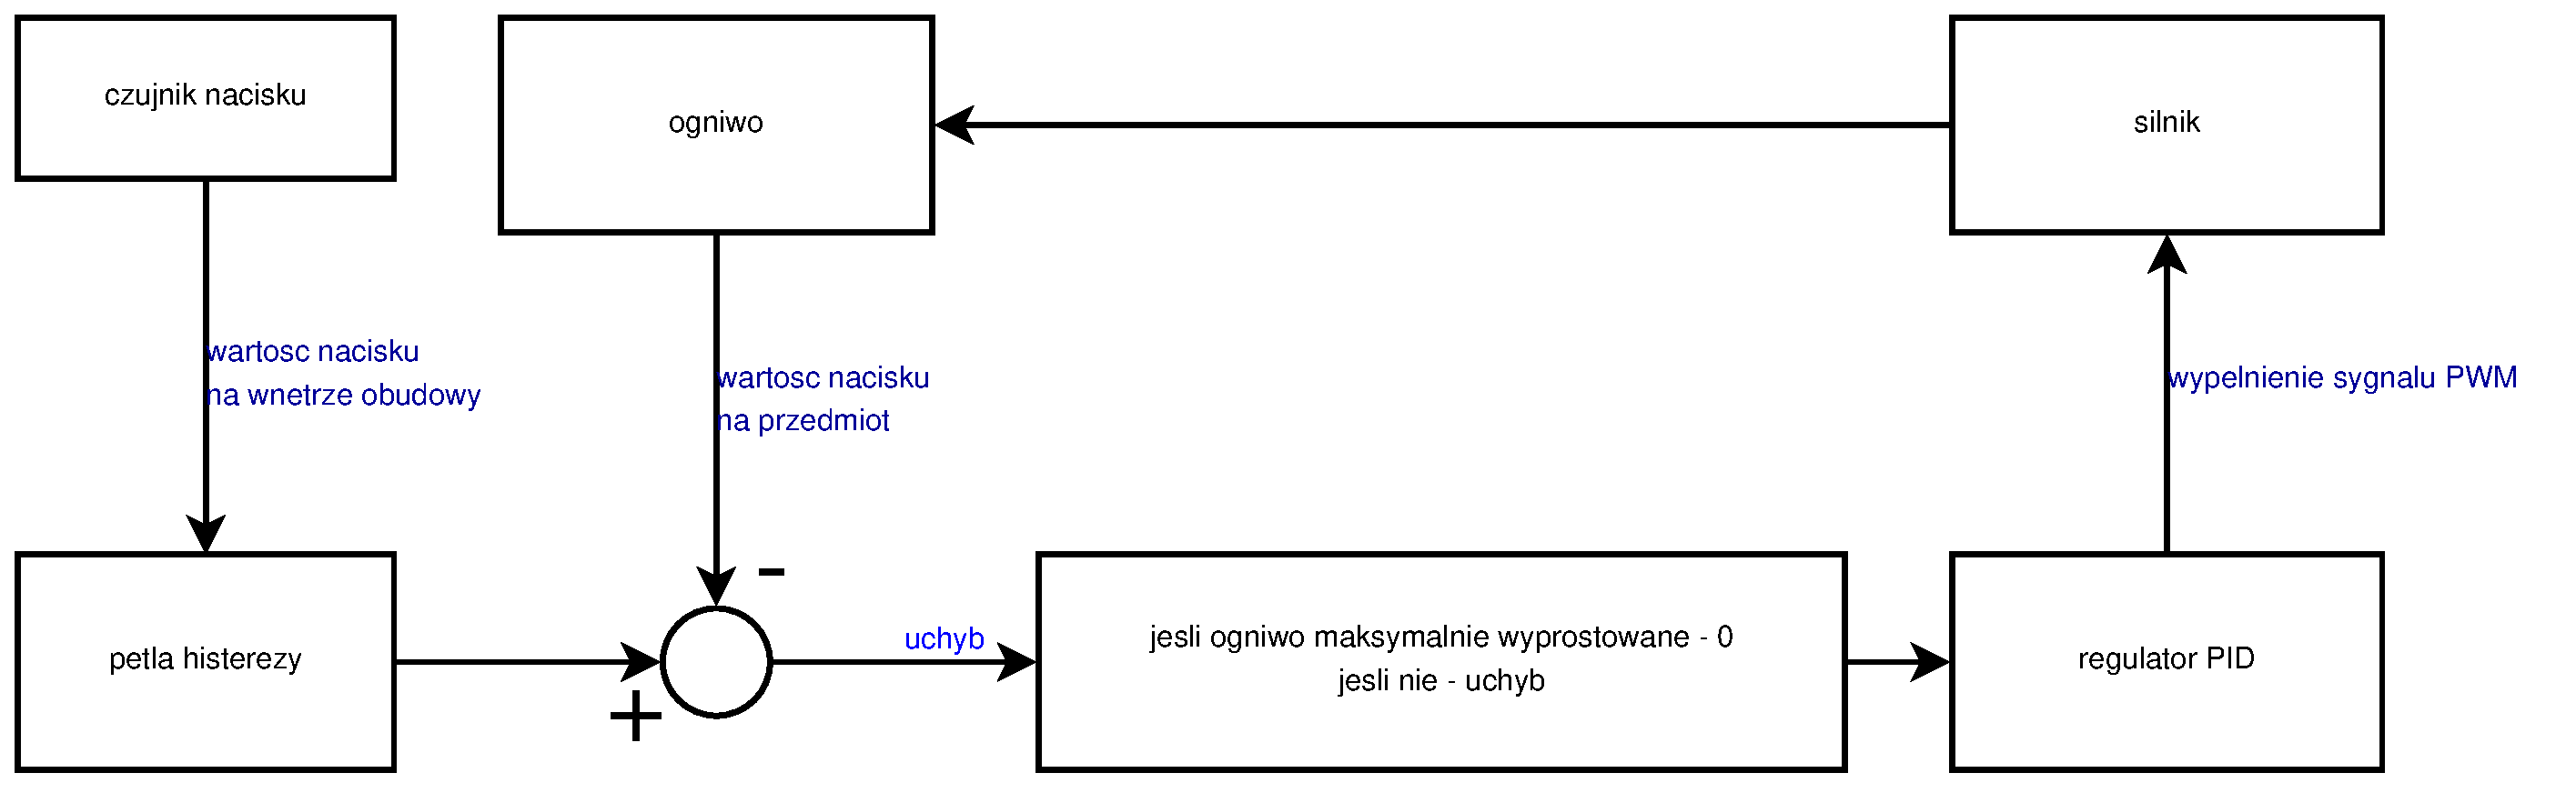
\includegraphics[width=12cm]{schemat_blokowy_algorytmu.eps}
\caption{Schemat blokowy proponowanego algorytmu}
\end{figure}


\item Sensory:

Do badania siły nacisku wykorzystamy okrągłe czujniki nacisku
\href{http://www.trossenrobotics.com/productdocs/2010-10-26-DataSheet-FSR402-Layout2.pdf}{FSR-402}.
Do obsługi każdego palca wykorzystamy 8 czujników nacisku.\\
Ich rozmieszczenie jest następujące:
\begin{itemize}
\item dwa sensory po bokach paliczka dalszego,
\item dwa sensory na wierzchu i spodzie paliczka dalszego,
\item dwa sensory na wierzchu i spodzie paliczka środkowego,
\item dwa sensory na wierzchu i spodzie paliczka bliższego.
\end{itemize}
W przypadku kciuka ich rozmieszczenie będzie następujące:
\begin{itemize}
\item dwa sensory po bokach paliczka dalszego,
\item dwa sensory na wierzchu i spodzie paliczka dalszego,
\item dwa sensory na wierzchu i spodzie paliczka bliższego,
\item dwa sensory na wierzchu i spodzie kości śródręcza.
\end{itemize}
Nakleimy je na wnętrze rękawicy, a ich końcówki zostaną od razu wyprowadzone na zewnątrz tak aby podczas wsadzania i wyciągania ręki nie zahaczyć o nie. Ich specyfikacja techniczna znajduje się w załączonym pliku o nazwie 2010-10-26-DataSheet-FSR402-Layout2.pdf. Wyjścia będą podłączone do przetwornika ADC w mikrokontrolerze.

Dodatkowo zastosujemy czujniki stykowe. Po osiągnięciu przez ruchome elementy granic swojego ruchu czujniki stykowe dostarczą informacji o tym zdarzeniu do mikrokontrolera i w razie potrzeby silniki zostaną zatrzymane.

Schemat z rozmieszczeniem sensorów zostanie wykonany i wysłany przy kolejnej aktualizacji raportu.

\item Zasilanie:

Przewidujemy użycie dwóch niezależnych źródeł zasilania. Jedno źródło zasilania będzie obsługiwać mikroprocesory, a drugie mostki H.
Silniki planujemy połączyć równolegle do źródła zasilania.

Moc wszystkich silników w najlepszym przypadku: \\
\begin{math}
3V \cdot 0.23A \cdot 20 silników = 13.8W
\end{math} \\
Moc wszystkich silników w najgorszym przypadku: \\
\begin{math}
3V \cdot 0.85A \cdot 20 silników = 51W
\end{math}

W takiej sytuacji potrzebujemy akumulatora o pojemności równej ok. 13.8Ah, zakładając że jej napięcie przez spadek napięcia na mostach H będzie musiało wynosić 3.7V. Mostki H będą połączone z GPIO do sterowania kierunkiem obrotu silników oraz z PWM do sterowania momentem obrotu.

Zależnie od doboru taktowania mikrokontrolera (1,4,25,40 MHz) oraz dobranego napięcia zasilania (2,3,4.2,5 V) pobór prądu będzie się różnić. Informacje odnośnie poboru prądu znajdują się w załączonej specyfikacji mikrokontrolera w rozdziale 26 na stronie 335. Po ustaleniu wymaganego taktowania mikrokontrolera odpowiedniego do obsługi wgranego programu zostanie przez nas dobrane zasilanie dla wszystkich mikrokontrolerów.

\item Konstrukcja rękawicy:

Do wykonania konstrukcji rękawicy planujemy użyć włókna węglowego. Do połączeń między czujnikami, mostkami, mikroprocesorami i zasilaniem wykorzystamy przewody miedziane z racji ich plastyczności. Propozycja konstrukcji rękawicy pojawi się po osiągnięciu II kamienia milowego.

\end{enumerate}

\end{document}